%%%%%%%%%%%%%%%%%%%%%%%%%%%%%%%%%%%%%%%%%%%%%%%%%%%%%%%%%%%%%%%%%
%  _____       ______   ____									%
% |_   _|     |  ____|/ ____|  Institute of Embedded Systems	%
%   | |  _ __ | |__  | (___    Wireless Group					%
%   | | | '_ \|  __|  \___ \   Zuercher Hochschule Winterthur	%
%  _| |_| | | | |____ ____) |  (University of Applied Sciences)	%
% |_____|_| |_|______|_____/   8401 Winterthur, Switzerland		%
%																%
%%%%%%%%%%%%%%%%%%%%%%%%%%%%%%%%%%%%%%%%%%%%%%%%%%%%%%%%%%%%%%%%%

\chapter{\textit{testbench}}\label{chap.testen}
Inspiriert vom Konzept des \textit{test driven development} wird stets parallel zur Entwicklung einer \textit{unit} (im folgenden als Block genannt) der \textit{unit-test} entwickelt.\textbf{(Kent, 2013)} \\

Nachdem im Voraus die Schnittstellen zwischen den Blocks geklärt sind (\textbf{siehe Kapitel xXX}) wird eine leere Hülle für jeden zu entwickelnden Block erstellt. Die \textit{testbench} geht von Beginn weg vom Ziel, ein funktionstüchtiges \textit{midi interface} aus. Solange ein Block nicht funktionert, werden die zu testenden Signale direkt an den Ausgang der DUT geführt.\\

\begin{figure}[H]
	\centering
	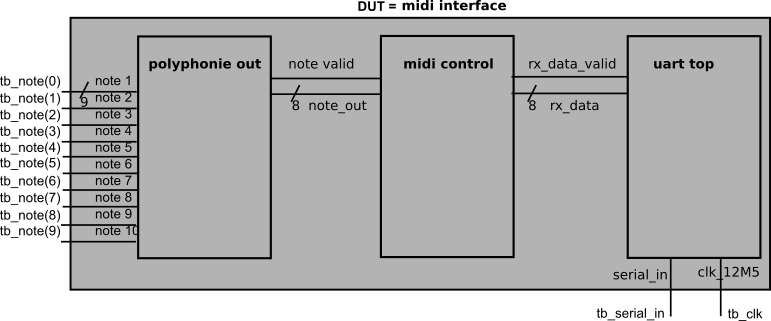
\includegraphics[width=1\textwidth]{images/midi_interface/testbench_midiinterface.png}
	\caption{Blockschaltbild Device under Test}
	\label{fig.testbench}
\end{figure}


In den nächsten zwei Unterkapiteln wird die Umsetzung der test driven Entwicklung beschrieben.\\


\section{unit test midi control}\label{sec.midi_control}


\section{unit test midi interface}\label{sec.midi_interface}



